% ======================================= %
% BRANCHING
% ======================================= %

\section[Branching]{Git Branches}

\begin{frame}
\frametitle{\large What is Branching?}
\begin{itemize}
\item Pretty much every version control system has some form of branching. This means that you diverge from the main line of development and continue to do work without changing the main line.
\pause
\item Usually this is an expensive process because you have to copy all of the source code in the directory into a new branch.
\pause
\item However, branching is where git truly shines. The git branch is extremely lightweight. This encourages branching in order to add new features.
\end{itemize}
\end{frame}

\begin{frame}
\frametitle{\large How Does Branching Work?}
\begin{center}
Let's look at a couple of examples from Pro Git (2nd Edition). \\
This book is licensed under the Creative Commons Attribution Non-Commercial Share Alike 3.0 License.
\end{center}
\end{frame}

\begin{frame}
\frametitle{\large How Does Branching Work?}
\begin{center}
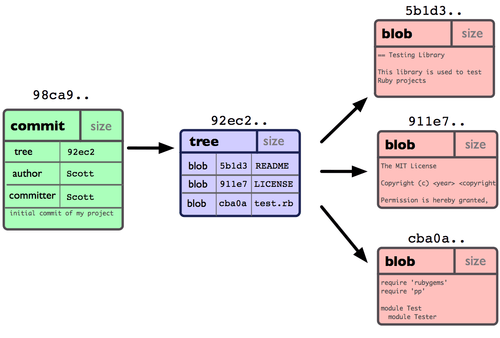
\includegraphics[width=0.55\textwidth]{img/branching_images/fig1.png}
\end{center}
\vspace{2mm}
\begin{center}
This is the structure of a commit.
\end{center}
\end{frame}

\begin{frame}
\frametitle{\large How Does Branching Work?}
\begin{center}
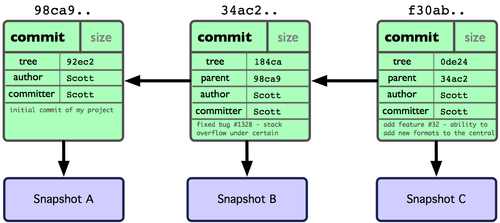
\includegraphics[width=0.55\textwidth]{img/branching_images/fig2.png}
\end{center}
\vspace{2mm}
\begin{center}
\# Add Code; git commit \\
\# Add Code; git commit \\
\# Add Code; git commit
\end{center}
\end{frame}

\begin{frame}
\frametitle{\large How Does Branching Work?}
\begin{center}
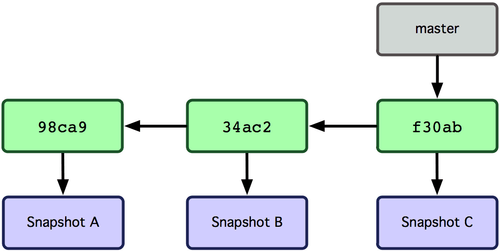
\includegraphics[width=0.55\textwidth]{img/branching_images/fig3.png}
\end{center}
\vspace{2mm}
\begin{center}
Every project starts off with a master branch.
\end{center}
\end{frame}

\begin{frame}
\frametitle{\large How Does Branching Work?}
\begin{center}
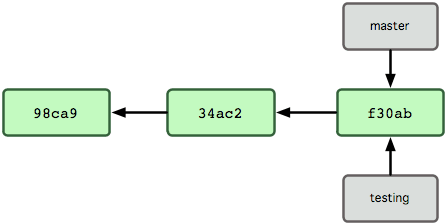
\includegraphics[width=0.55\textwidth]{img/branching_images/fig4.png}
\end{center}
\vspace{2mm}
\begin{center}
git branch testing
\end{center}
\end{frame}

\begin{frame}
\frametitle{\large How Does Branching Work?}
\begin{center}
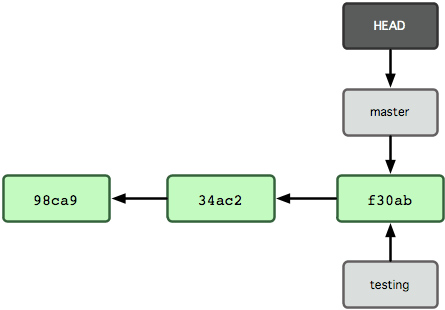
\includegraphics[width=0.55\textwidth]{img/branching_images/fig5.png}
\end{center}
\vspace{2mm}
\begin{center}
HEAD is still on the master branch.
\end{center}
\end{frame}

\begin{frame}
\frametitle{\large How Does Branching Work?}
\begin{center}
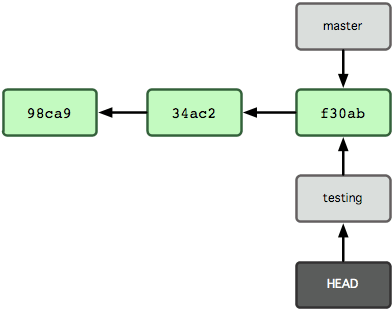
\includegraphics[width=0.55\textwidth]{img/branching_images/fig6.png}
\end{center}
\vspace{2mm}
\begin{center}
git checkout testing
\end{center}
\end{frame}

\begin{frame}
\frametitle{\large How Does Branching Work?}
\begin{center}
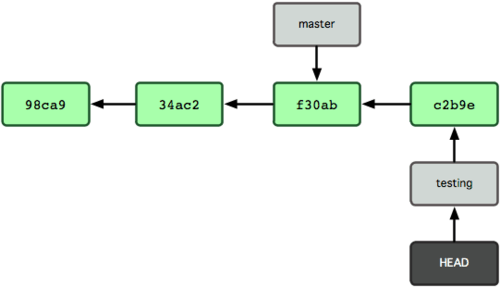
\includegraphics[width=0.55\textwidth]{img/branching_images/fig7.png}
\end{center}
\vspace{2mm}
\begin{center}
\# Add New Code to testing Branch\\
git commit
\end{center}
\end{frame}

\begin{frame}
\frametitle{\large How Does Branching Work?}
\begin{center}
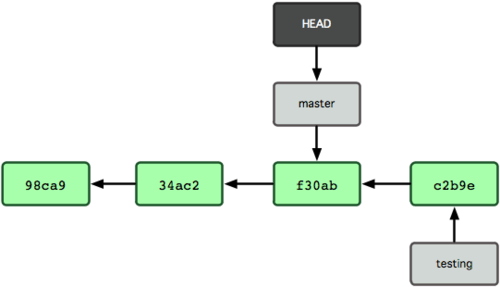
\includegraphics[width=0.55\textwidth]{img/branching_images/fig8.png}
\end{center}
\vspace{2mm}
\begin{center}
git checkout master
\end{center}
\end{frame}

\begin{frame}
\frametitle{\large How Does Branching Work?}
\begin{center}
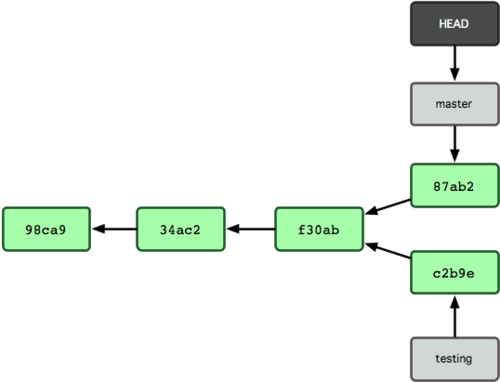
\includegraphics[width=0.55\textwidth]{img/branching_images/fig9.png}
\end{center}
\vspace{2mm}
\begin{center}
Add New Code to Master \\
git commit
\end{center}
\end{frame}

\begin{frame}
\frametitle{\large How Does Merging Work?}
\begin{center}
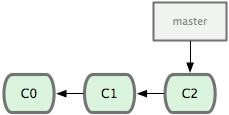
\includegraphics[width=0.55\textwidth]{img/branching_images/f1.png}
\end{center}
\vspace{2mm}
\begin{center}
Suppose we have a project with a few current commits.
\end{center}
\end{frame}

\begin{frame}
\frametitle{\large How Does Merging Work?}
\begin{center}
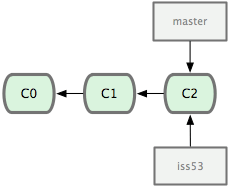
\includegraphics[width=0.55\textwidth]{img/branching_images/f2.png}
\end{center}
\vspace{1mm}
\begin{center}
\small git checkout -b iss53 \\
\small (git branch iss53; git checkout iss53)
\end{center}
\end{frame}

\begin{frame}
\frametitle{\large How Does Merging Work?}
\begin{center}
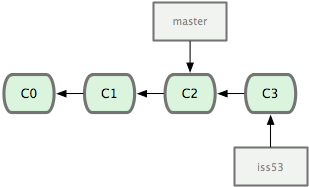
\includegraphics[width=0.55\textwidth]{img/branching_images/f3.png}
\end{center}
\vspace{2mm}
\begin{center}
\# Add Code to iss53 Branch \\
git commit
\end{center}
\end{frame}

\begin{frame}
\frametitle{\large How Does Merging Work?}
\begin{center}
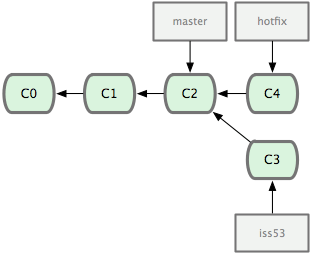
\includegraphics[width=0.45\textwidth]{img/branching_images/f4.png}
\end{center}
\begin{center}
\small git checkout master \\
\small git checkout -b hotfix \\
\small Add code to hotfix branch \\
\small git commit
\end{center}
\end{frame}

\begin{frame}
\frametitle{\large How Does Merging Work?}
\begin{center}
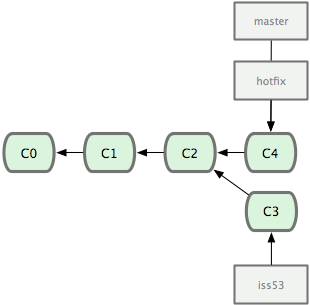
\includegraphics[width=0.4\textwidth]{img/branching_images/f5.png}
\end{center}
\vspace{2mm}
\begin{center}
\small git checkout master \\
\small git merge hotfix \\
\small git branch -d hotfix
\end{center}
\end{frame}

\begin{frame}
\frametitle{\large How Does Merging Work?}
\begin{center}
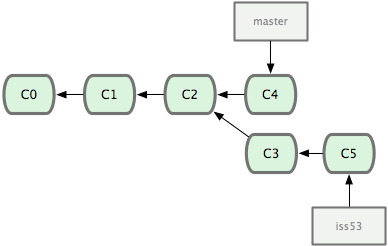
\includegraphics[width=0.55\textwidth]{img/branching_images/f6.png}
\end{center}
\vspace{2mm}
\begin{center}
git checkout iss53 \\
\# Add code to iss53 branch \\
git commit
\end{center}
\end{frame}

\begin{frame}
\frametitle{\large How Does Merging Work?}
\begin{center}
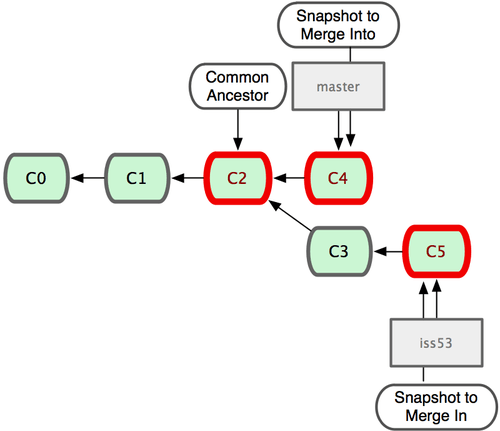
\includegraphics[width=0.55\textwidth]{img/branching_images/f7.png}
\end{center}
\vspace{2mm}
\begin{center}
We want to merge iss53 to master
\end{center}
\end{frame}

\begin{frame}
\frametitle{\large How Does Merging Work?}
\begin{center}
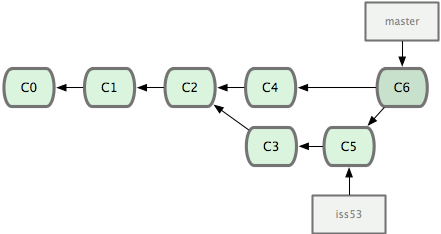
\includegraphics[width=0.55\textwidth]{img/branching_images/f8.png}
\end{center}
\vspace{2mm}
\begin{center}
git checkout master \\
git merge iss53
\end{center}
\end{frame}

\begin{frame}
\frametitle{\large Merge Conflicts}
\begin{center}
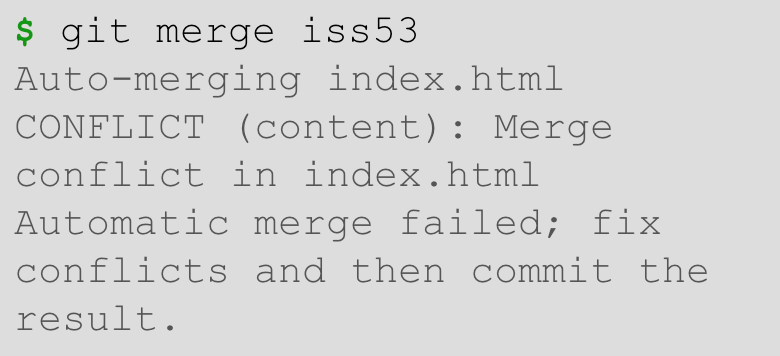
\includegraphics[width=0.55\textwidth]{img/branching_images/merge1.png}
\end{center}
\vspace{2mm}
\begin{center}
Sometimes we run into merge conflicts.
\end{center}
\end{frame}

\begin{frame}
\frametitle{\large Merge Conflicts}
\begin{center}
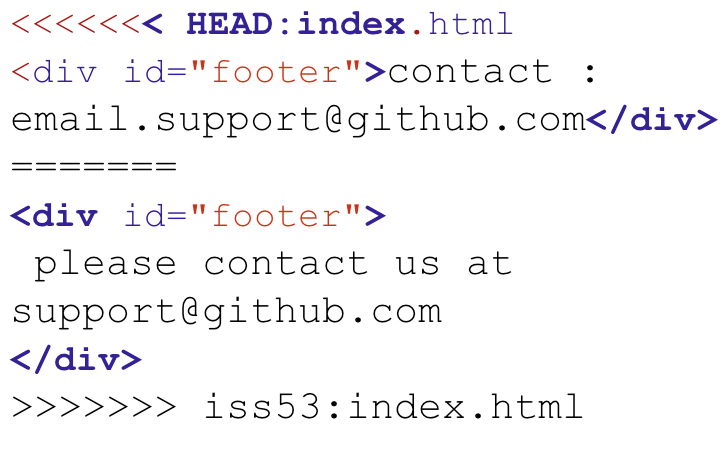
\includegraphics[width=0.55\textwidth]{img/branching_images/merge2.png}
\end{center}
\vspace{2mm}
\begin{center}
The ``======'' divides the two types of code.
\end{center}
\end{frame}